\subsection{Portfolio accounting}
\label{sec:framework}

Strategies receive dated market history and prior targets, then return weights
and a decision audit. One ledger handles execution, financing and corporate
actions across strategies. Execution can refill the saved ranking without
recomputing signals from later observations.

\begin{figure}[H]
\centering
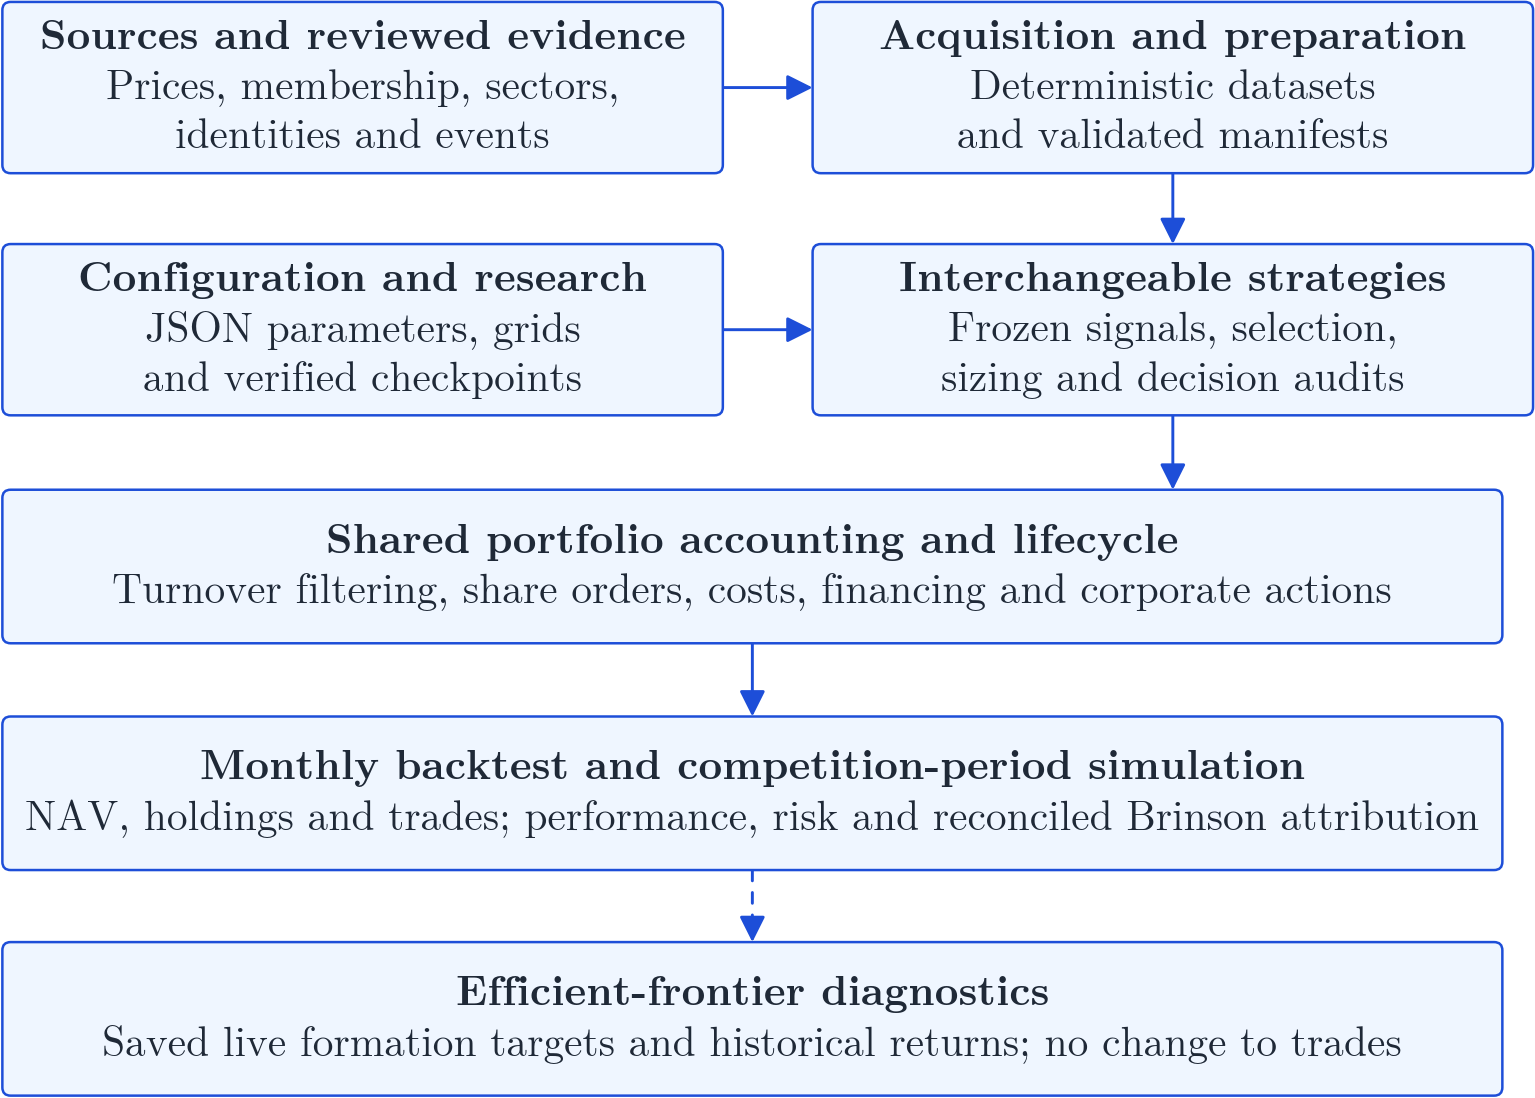
\includegraphics[width=\reportfigurewidth]{figures/framework_architecture.png}
\caption[Framework architecture]{The shared framework. The dashed connection is a diagnostic;
frontier allocations do not enter the trading simulation.}
\label{fig:architecture}
\end{figure}

For cash $C_t$, restricted short proceeds $R_t$, signed units $n_{i,t}$ and
prices $P_{i,t}$, the ledger gives NAV, free cash $F_t$ and borrowing $L_t$:
\begin{equation}
  \operatorname{NAV}_t=C_t+\sum_i n_{i,t}P_{i,t},\qquad
  F_t=C_t-R_t,\qquad L_t=\max(-F_t,0).
\label{eq:ledger}
\end{equation}

Positive free cash earns 2\%; negative free cash incurs 8\%, compounded on
Actual/365 days. Execution enforces whole-unit orders, position counts and the
gross ceiling. Buys and covers pay the ask; sales and shorts receive the bid,
with a modeled half-spread of 1-15 basis points. Each order costs \$2;
a sign reversal has two charged legs.

Resolved JSON parameters and assumptions accompany each run. Searches retain
rejected, duplicate, history-unready, infeasible and ranked cases separately;
candidate numbers are grid-relative. Resume verifies parameters, data, source
bytes, runtime versions and output hashes. Tests cover accounting, corporate
actions, construction, future-data isolation, identities, checkpoints and
attribution.

\subsection{Performance measurement}
\label{sec:performance-metrics}

For aligned periodic portfolio, benchmark and risk-free returns \(r_p,r_b,r_f\),
we use sample standard deviations (\(n-1\) denominator), with \(k=12\) for
monthly history and \(k=252\) for daily competition risk:
\begin{align}
 \sigma_{\mathrm{ann}}&=\sqrt{k}\,s(r_p),&
 \mathrm{Sharpe}&=\sqrt{k}\,\frac{\overline{r_p-r_f}}{s(r_p-r_f)},\\
 \mathrm{IR}&=\sqrt{k}\,\frac{\overline{r_p-r_b}}{s(r_p-r_b)},&
 \mathrm{Treynor}&=\frac{k\,\overline{r_p-r_f}}{\widehat{\beta}}.
\end{align}
OLS estimates \(r_p-r_f=\alpha+\beta(r_b-r_f)+\varepsilon\);
reported annual alpha is \(k\widehat{\alpha}\). Annualized compound return uses NAV growth,
whereas these ratios use arithmetic excess means
\citep{sharpe1994,kidd2011}. Maximum drawdown is
\(\min_t[\mathrm{NAV}_t/\max_{s\le t}\mathrm{NAV}_s-1]\).
